\documentclass[../main.tex]{subfiles}
%\usepackage{import}

\begin{document}

\setlength{\delimitershortfall}{0pt}

\section{Numerical solution}\label{sec:finite_volume_method}
\subsection{General}
Like \ac{FD} or \acf{FE}, the \acf{FV} method is a mean of solving a \ac{PDE} by transforming it into a discrete algebraic form. In the field of fluid mechanics, the finite volume method is the most popular approach. Other than \ac{FD} or \ac{FE}, the \ac{FV} is conservative by construction. In contrast to \ac{FD} it can easily be implemented for unstructured grids. Compared to the \ac{FE} method, where boundary conditions come naturally from the formulation, this causes some difficulties in \ac{FV}.\\
It shall also be mentioned that the introduction of stabilization schemes(like streamline upwinding), is much easier in an \ac{FV} formulation.
Overall, for \ac{CFD}, \ac{FV} has so far shown to be the best compromise between accuracy, stability and efficiency.
 \\
 \\
Finite volume methods are typically derived from the so called conservative form of a \ac{PDE}. It is shown in Section~\ref{sec:conservative_form_nsg}, that the \ac{NSE} equation can be  brought to the conservative form. In general, the conservative form can be written as:
\begin{align}\label{eq:general_conservative_form}
\tfrac{\vec{\xi}}{t}+\nabla\cdot f(\vec{\xi}) = \vec{0} \\
\end{align}
where $\vec{\xi}$ represents a vector of states and $f$ is the so-called flux tensor.\\
After subdividing the domain into finite volumes, also called cells, one can write for each particular cell $i$
\begin{align}
\int_{V_i} \tfrac{\vec{\xi}}{t} dV_i + \int_{V_i} \nabla\cdot f(\vec{\xi}) dV_i
\end{align}
It shall be stressed again that reformulating the equations in integral form has already changed the space of admissible solutions. Particularly, the integral form is capable of capturing discontinuities, like shocks whereas the derivative term would be undefined  at a shock in equation \eqref{eq:general_conservative_form}.

After applying the divergence theorem to the second term this gives:
\begin{align}
\tfrac{~}{t}\int_{V_i} \vec{\xi} dV_i + \int_{\partial V_i} f(\vec{\xi})\cdot\normal~dS_i
\end{align}
And after integration the first term to get the volume average
\begin{align}
V_i \tfrac{\dvec{\bar{\xi}}}{t} + \int_{\partial V_i} f(\vec{\xi})\cdot\normal~dS_i
\end{align}
So that finally, the equation can be written as
\begin{align}\label{eq:final_fv_general}
\tfrac{\dvec{\bar{\xi}}}{t} + \frac{1}{V_i} \int_{\partial V_i} f(\vec{\xi})\cdot\normal~dS_i
\end{align}
which can easily be interpreted: The cell average of the conserved properties changes according to the total flux through the cells surface.
Of course, the conservative value is defined as being constant within one cell, so there will be different values on faces or edges, depending on which side one is looking at. There are different approaches on how to choose an appropriate value, and the choice may greatly effect the numerical properties. In a \ac{FV} solver, the numerical flux at the interface is typically constructed such, that upwinding is achieved.

\subsection{Finite Volume method for fluid mechanics}\label{sec:fv_fluid_mechanics}
It has already been shown in Section~\ref{sec:conservative_form_nsg}, that the \ac{NSE} can be brought into the conservative form~\eqref{eq:nsg_conservative_form}. The flux has been shown to consist of a convective and a diffusive part\eqref{eq:fluxesconv}\eqref{eq:fluxes_diff}.
For this thesis, a \ac{MUSCL} type \ac{FV} framework for unstructured three-dimensional grids, as described in~\cite{Main2014} has been used.



In equivalent manner as in equations \eqref{eq:general_conservative_form} to \eqref{eq:final_fv_general} one can now write the conservative form of the \ac{NSE} as

\begin{align}\label{eq:NSE_full_FV formulation}
\pdfrac{\bar{\fstate_i}}{t} +
\frac{1}{\norm{\Omega_i}} \int_{\partial\Omega_i} \fluxesconv(\fstate)\cdot dS +
\frac{1}{\norm{\Omega_i}} \int_{\partial\Omega_i} \fluxesdiff(\fstate,\nabla \fstate)\cdot dS =
\vec{0}
\end{align}


\subsection{Mixed \ac{FV}-\ac{FE} formulation}\label{sec:mixed_FV_FE_formulation}
It would be totally feasible to now solve both terms with classical \ac{FV} methods. However, we note two things. First, there is no need for upwinding in the diffusive term due to its elliptic nature.
Secondly, the integration of the second term also becomes much more cumbersome than the first one due to the gradient of the fluid state vector demanding at least a first order representation.\\
For this reasons, we introduce the following, mixed \ac{FV}-\ac{FE} formulation

\begin{align}\label{eq_mixed_FV_FE}
\pdfrac{\fstate_i}{t} +
\int_{\partial\dualcell_i} \fluxesconv(\fstate)\cdot dS -
\int_{\sum_{T_i}} \difftensor \fstate \nabla \phi_i dx =
\vec{0}
\end{align}

where $\difftensor$ is the diffusive tensor introduced in \textbf{TODO} and $\phi_i$ is a linear P1 shape-function over the triangle.
Please also note that the convective term is now integrated over the dual cell related to vertex $i$, whereas the diffusive term integrated over all primal triangles connected to vertex $i$.\\
We will justify this re-formulation in section~\ref{sec:viscous_term_treatment}. See also figure~\ref{fig:dualcell_unstructured}.







%The formulation is derived by re-writing equation~\ref{eq:nsg_conservative_form} in variational form by multiplying with a test function:
%\begin{align}
%\int_\Omega \pdfrac{\fstate}{t}\testfunc_i d\Omega +
%\int_\Omega \nabla\cdot\fluxesconv(\fstate)\testfunc_i d\Omega +
% \int_{\Omega} \nabla\cdot\fluxesdiff(\fstate)\testfunc_i d\Omega = \vec{0}
%\end{align}
%where $\testfunc_i \in C^0(\Omega)$. For this formulation $\testfunc_i$ is chosen to be piecewise linear. Particularly, the test functions fulfill
%\begin{align}
%\testfunc_i(\vertex_j)=\delta_{ij}
%\end{align}
%Now, Gauss divergence theorem is applied to the last part, giving
%\begin{align}
%\int_\Omega \pdfrac{\fstate}{t}\testfunc_i ~d\Omega +
%\int_\Omega \nabla\cdot\fluxesconv(\fstate)\testfunc_i ~d\Omega +
%\left(
%  \int_{\Gamma} \fluxesdiff(\fstate)\cdot\normal ~d\Gamma - \int_\Omega \fluxesdiff(\fstate)\cdot\nabla\testfunc_i ~d\Omega
%\right)
%=\vec{0}
%\end{align}
%In contrast to a real \ac{FE} formulation, the contribution of the viscous flux at the far field boundary is now neglected, as explained in \cite{Lakshminarayan2014}. How the boundary conditions at the far fields are taken care of will be explained at a proper place.
%We finally get the mixed \ac{FV}-\ac{FE} form by mass lumping the first two terms. Since we are using a vertex-centered approach here, mass lumping is equivalent to using a constant test function of $\testfunc_i$ on the dual cell. We therefore get:
%\begin{align}
%\int_{\Omega_i} \pdfrac{\fstate}{t} ~d\Omega +
%\int_{\Omega_i} \nabla\cdot\fluxesconv(\fstate) ~d\Omega -
%\int_\Omega \fluxesdiff(\fstate)\cdot\nabla\testfunc_i ~d\Omega  =
%\vec{0}
%\end{align}
%Please note that we have switched from an integral over the whole domain to an integral across the dual cells here.
%Finally by averaging $\fstate$ over the cell in the first term, we can derive the \ac{FV} formulation as
%\begin{align}
%\pdfrac{\fstate_i}{t} +
%\frac{1}{\norm{\Omega_i}} \int_{\Omega_i} \nabla\cdot\fluxesconv(\fstate) ~d\Omega_i -
%\frac{1}{\norm{\Omega_i}} \int_\Omega \fluxesdiff(\fstate)\cdot\nabla\testfunc_i ~d\Omega  =
%\vec{0}
%\end{align}
%Where now, $\fstate_i$ denotes the average of $\fstate$ in the dual cell $\Omega_i$, which is by construction the value of $\fstate$ at vertex $i$. The volume of cell $\Omega_i$ is denoted as $\norm{\Omega_i}$ here.
%Finally, gauss divergence theorem is applied to the convective term, resulting in
%\begin{align}\label{eq:nsg_basic_fv-form}
%\pdfrac{\fstate_i}{t} +
%\frac{1}{\norm{\Omega_i}} \int_{\partial\Omega_i} \fluxesconv(\fstate)\cdot dS -
%\frac{1}{\norm{\Omega_i}} \int_\Omega \fluxesdiff(\fstate)\cdot\nabla\testfunc_i ~d\Omega  =
%\vec{0}
%\end{align}
\vskip 1cm 
As can be seen from Figure \ref{fig:dualcell_unstructured}, the dual cells themselves can have very random shapes. This makes the integration over the boundary of the second term in Equation \eqref{eq_mixed_FV_FE} more cumbersome than in a primal approach. Also, the volume integral in the \ac{FE}-like expression has to be splitted into regular shaped subdomains, e.g. tetrahedra, such that standard integration rules, like gauss-rule, can be applied.




\begin{figure}[h]
  \centering
  \scalebox{.75}{\documentclass[../../main.tex]{subfiles}
%\usepackage{import}
\usepackage{pdftricks}
\begin{document}
\setlength{\delimitershortfall}{0pt}

%LaTeX with PSTricks extensions
%%Creator: inkscape 0.91
%%Please note this file requires PSTricks extensions
\psset{xunit=.5pt,yunit=.5pt,runit=.5pt}
\begin{pspicture}(309.21918013,431.058343)
{
\newrgbcolor{curcolor}{0 0 0}
\pscustom[linewidth=2,linecolor=curcolor]
{
\newpath
\moveto(1.54615,159.693858)
\lineto(183.96406,22.148808)
\lineto(307.85215,127.502468)
\lineto(165.91737,315.285608)
\closepath
}
}
{
\newrgbcolor{curcolor}{0 0 0}
\pscustom[linewidth=2,linecolor=curcolor]
{
\newpath
\moveto(182.98856,22.636558)
\lineto(165.91737,314.797858)
}
}
{
\newrgbcolor{curcolor}{0 0 0}
\pscustom[linewidth=2,linecolor=curcolor,linestyle=dashed,dash=8 8]
{
\newpath
\moveto(307.36441,127.990208)
\lineto(1.54615,159.693858)
}
}
{
\newrgbcolor{curcolor}{0 0 0}
\pscustom[linestyle=none,fillstyle=solid,fillcolor=curcolor]
{
\newpath
\moveto(177.49793992,322.71041737)
\lineto(179.07020555,322.71041737)
\lineto(179.07020555,313.14010487)
\lineto(177.49793992,313.14010487)
\lineto(177.49793992,322.71041737)
\closepath
\moveto(177.49793992,326.4360033)
\lineto(179.07020555,326.4360033)
\lineto(179.07020555,324.44503651)
\lineto(177.49793992,324.44503651)
\lineto(177.49793992,326.4360033)
\closepath
}
}
{
\newrgbcolor{curcolor}{0 0 0}
\pscustom[linestyle=none,fillstyle=solid,fillcolor=curcolor]
{
\newpath
\moveto(185.49793992,13.21044788)
\lineto(187.07020555,13.21044788)
\lineto(187.07020555,3.46923695)
\curveto(187.07020555,2.25016143)(186.83664435,1.36718617)(186.36952195,0.82031117)
\curveto(185.90809617,0.27343617)(185.16183966,-0.00000133)(184.13075242,-0.00000133)
\lineto(183.53260789,-0.00000133)
\lineto(183.53260789,1.33300648)
\lineto(183.95130906,1.33300648)
\curveto(184.54945359,1.33300648)(184.95676154,1.47257354)(185.17323289,1.75170765)
\curveto(185.38970424,2.02514515)(185.49793992,2.59765492)(185.49793992,3.46923695)
\lineto(185.49793992,13.21044788)
\closepath
\moveto(185.49793992,16.93603382)
\lineto(187.07020555,16.93603382)
\lineto(187.07020555,14.94506702)
\lineto(185.49793992,14.94506702)
\lineto(185.49793992,16.93603382)
\closepath
}
}
{
\newrgbcolor{curcolor}{0.7019608 0.7019608 0.7019608}
\pscustom[linestyle=none,fillstyle=solid,fillcolor=curcolor,opacity=0.47058824]
{
\newpath
\moveto(78.12265,233.343868)
\lineto(105.92431,177.740548)
\lineto(174.69684,164.571338)
\lineto(221.03294,167.985578)
\lineto(244.93261,210.419698)
\lineto(156.65015,196.274988)
\closepath
}
}
{
\newrgbcolor{curcolor}{0 0 0}
\pscustom[linewidth=1,linecolor=curcolor]
{
\newpath
\moveto(78.12265,233.343868)
\lineto(105.92431,177.740548)
\lineto(174.69684,164.571338)
\lineto(221.03294,167.985578)
\lineto(244.93261,210.419698)
\lineto(156.65015,196.274988)
\closepath
}
}
{
\newrgbcolor{curcolor}{0 0 0}
\pscustom[linewidth=1,linecolor=curcolor]
{
\newpath
\moveto(156.1624,196.762738)
\lineto(157.71186,160.154558)
\lineto(105.92431,177.740548)
}
}
{
\newrgbcolor{curcolor}{0 0 0}
\pscustom[linewidth=1,linecolor=curcolor]
{
\newpath
\moveto(157.13789,160.181608)
\lineto(220.54519,167.497838)
}
}
{
\newrgbcolor{curcolor}{0 0 0}
\pscustom[linewidth=1,linecolor=curcolor]
{
\newpath
\moveto(174.45296,164.693278)
\lineto(157.62564,160.425478)
}
}
{
\newrgbcolor{curcolor}{0.7019608 0.7019608 0.7019608}
\pscustom[linestyle=none,fillstyle=solid,fillcolor=curcolor,opacity=0.47058824]
{
\newpath
\moveto(136.07914,168.120158)
\curveto(124.61423,172.012978)(115.341,175.217608)(115.47195,175.241548)
\curveto(115.6029,175.265448)(124.29799,173.512428)(135.59085,171.382448)
\lineto(157.57506,167.235958)
\lineto(157.74744,160.828918)
\lineto(136.07907,168.120158)
\closepath
}
}
{
\newrgbcolor{curcolor}{0.7019608 0.7019608 0.7019608}
\pscustom[linestyle=none,fillstyle=solid,fillcolor=curcolor,opacity=0.47058824]
{
\newpath
\moveto(157.57684,167.205298)
\curveto(157.79026,167.156898)(161.49733,166.503048)(164.76988,165.883728)
\curveto(168.04245,165.264408)(170.8597,164.700228)(171.03045,164.629998)
\curveto(171.23246,164.546898)(169.02941,164.029218)(164.80386,162.844628)
\lineto(157.74516,160.865788)
\lineto(157.57684,167.205298)
\closepath
}
}
{
\newrgbcolor{curcolor}{0.7019608 0.7019608 0.7019608}
\pscustom[linestyle=none,fillstyle=solid,fillcolor=curcolor,opacity=0.47058824]
{
\newpath
\moveto(170.2027,162.964188)
\lineto(174.68628,164.061608)
\lineto(187.18855,164.937858)
\curveto(194.06479,165.419788)(199.80722,165.802938)(199.94948,165.789288)
\curveto(200.32737,165.752988)(166.8486,161.850248)(166.23646,161.859208)
\curveto(165.95193,161.863208)(167.73674,162.360608)(170.2027,162.964188)
\closepath
}
}
{
\newrgbcolor{curcolor}{0 0 0}
\pscustom[linestyle=none,fillstyle=solid,fillcolor=curcolor]
{
\newpath
\moveto(168.59877,315.07760487)
\curveto(168.59877,313.5933396)(167.39553526,312.39010487)(165.91127,312.39010487)
\curveto(164.42700474,312.39010487)(163.22377,313.5933396)(163.22377,315.07760487)
\curveto(163.22377,316.56187013)(164.42700474,317.76510487)(165.91127,317.76510487)
\curveto(167.39553526,317.76510487)(168.59877,316.56187013)(168.59877,315.07760487)
\closepath
}
}
{
\newrgbcolor{curcolor}{0 0 0}
\pscustom[linewidth=1,linecolor=curcolor]
{
\newpath
\moveto(77.6349,234.319368)
\lineto(37.63953,296.263418)
\lineto(87.87762,416.737278)
\lineto(214.69221,430.39423)
\lineto(265.90579,352.354488)
\lineto(303.46242,277.728978)
\lineto(245.42036,210.907438)
}
}
{
\newrgbcolor{curcolor}{0 0 0}
\pscustom[linewidth=1,linecolor=curcolor]
{
\newpath
\moveto(220.78906,167.741708)
\curveto(221.76456,167.985578)(303.21855,227.490888)(303.21855,227.490888)
\lineto(303.21855,277.728978)
}
}
{
\newrgbcolor{curcolor}{0 0 0}
\pscustom[linewidth=1,linecolor=curcolor]
{
\newpath
\moveto(37.28653,296.670418)
\lineto(24.1807,223.898578)
\lineto(106.26457,177.683298)
}
}
{
\newrgbcolor{curcolor}{0 0 0}
\pscustom[linewidth=1,linecolor=curcolor]
{
\newpath
\moveto(173.86305,164.577468)
\lineto(145.13492,324.655538)
\lineto(87.6405,417.037098)
}
}
{
\newrgbcolor{curcolor}{0 0 0}
\pscustom[linewidth=1,linecolor=curcolor]
{
\newpath
\moveto(144.30228,323.822908)
\curveto(145.68184,325.892248)(266.63852,351.163068)(266.63852,351.163068)
}
}
{
\newrgbcolor{curcolor}{0 0 0}
\pscustom[linewidth=1,linecolor=curcolor,linestyle=dashed,dash=3 3]
{
\newpath
\moveto(302.97467,228.466388)
\lineto(210.79022,283.581958)
\lineto(24.47032,223.588898)
}
}
{
\newrgbcolor{curcolor}{0 0 0}
\pscustom[linewidth=1,linecolor=curcolor,linestyle=dashed,dash=3 3]
{
\newpath
\moveto(23.83581,223.898578)
\lineto(75.22445,366.683128)
\lineto(184.20976,370.132028)
\lineto(211.1112,283.564588)
\lineto(156.27365,196.307368)
}
}
{
\newrgbcolor{curcolor}{0 0 0}
\pscustom[linewidth=1,linecolor=curcolor,linestyle=dashed,dash=3 3]
{
\newpath
\moveto(184.20976,370.132028)
\lineto(214.90499,430.83271)
}
}
{
\newrgbcolor{curcolor}{0 0 0}
\pscustom[linewidth=1,linecolor=curcolor,linestyle=dashed,dash=3 3]
{
\newpath
\moveto(210.76631,283.564588)
\lineto(266.63852,351.163068)
}
}
{
\newrgbcolor{curcolor}{0 0 0}
\pscustom[linewidth=1,linecolor=curcolor,linestyle=dashed,dash=3 3]
{
\newpath
\moveto(75.3969,367.028018)
\lineto(87.98539,416.864658)
}
}
\end{pspicture}

\end{document}}
  \caption[\ac{FV} semi-discretization of an unstructured mesh]{\ac{FV} semi-discretization of an unstructured mesh. Vertex $i$ is the center of dual cell $C_i$. The primal element is drawn in thick black lines, the dual cell in dashed lines. The boundary of the dual cell is denoted as $\pd C_{ij}$}
  \label{fig:dualcell_unstructured}
\end{figure}


For a closer look into the convective fluxes integral, we decompose the boundary as $\pd \Omega_i = \sum_{i \in \vertexset(i)} \pd\Omega_{ij}$, where $\vertexset(i)$ denotes the set of vertices connected by an edge to vertex $i$.\\
In this thesis, the surface integral in equation \eqref{eq_mixed_FV_FE} is then approximated using a Riemann solver~\cite{Roe1981} and a \ac{MUSCL} \cite{VanLeer1979} technique. This approximation can be written as
\begin{align}\label{eq:convectiveterm_approximation}
\int_{\partial\Omega_i} \fluxesconv(\fstate)\cdot dS \approx
\sum_{j \in \vertexset(i)} \fluxesnum_{ij}(\fstate_{ij},\fstate_{ji},\normal_{ij})
\end{align}
where $\fluxesnum_{ij}$ denotes the chosen numerical flux function along the edge $i-j$ and the two extrapolated fluid states at the $i$ and the $j$-side of the the intersection of the cell boundary $\partial \Omega_{ij}$ and edge $i-j$ are denoted by $\fstate_{ij}$ and $\fstate_{ji}$ respectively. The area-weighted normal of edge $i-j$ is denoted as $\normal_{ij}$.
 \\
 A popular choice for the numerical approximation of the convective fluxes is the so-called Roe flux. Appropriate upwinding is directly built into the definition of the Roe flux ~\cite{Roe1981}. In 1D it is defined as:
 \begin{align}
\fluxesnum_{ij}=\frac{1}{2} \left(\fluxesconv(\dfstate_j)+\fluxesconv(\dfstate_i) \right)-\frac{1}{2}\abs{
\dmat{A}} \left( \dfstate_j-\dfstate_i \right)
 \end{align}
where $\dmat{A}$ is the flux Jacobian.
 \\
To evaluate a roe-flux between two points in 2D or 3D, a normal vector is required to project the higher, dimensional flux on the connecting line.
\\
As for the volume integral of the diffusive term in Equation~\eqref{eq_mixed_FV_FE}, it shall be noted that the shape function is still defined in the primal cell. Since the gradient of the test function is constant, as is the diffusive flux itself, the integral becomes a summation of the primal sub-tetrahedral contributions.


The final numerical approximation can therefore be summarized as
\begin{align}\label{eq:nse_final_discretized}
\pdfrac{\bar{\dfstate_i}}{t} +
\sum_{j \in \vertexset(i)} \fluxesnum_{ij}(\dfstate_{ij},\dfstate_{ji},\wnormal_{ij}) -
\sum_{T_i \in \elementset(i)} \int_{T_j} \difftensor \nabla \dfstate \nabla \phi_j dx =
\vec{0}
\end{align}
where $\vertexset(i)$ is the set of vertices connected to vertex $i$ by an edge, and $\elementset(i)$ is the set of primal elements connected to vertex $i$.

%%%%%%%%%%%%%%%%%%%%%%%%%%%%%%%%%%%%%%%%%%%%%%%%%%%%%%%%%%%%%%%%%%%%%%%%%%%%%%%%%%%%%%%%%%%%%%%%%%%%%%%%%%%%%%%%%%%%%%%%%
\cleardoublepage
\subsection{Derivation of the mixed \ac{FV}-\ac{FE} formulation}\label{sec:viscous_term_treatment}
The equivalence of the finite volume representation of the viscous term, with the finite element-like representation provided in Equation \eqref{eq_mixed_FV_FE} might not be obvious to the reader. This section is therefore denoted to a \ac{FE} discretization of the governing equations, that can then be reformulated such that the mixed \ac{FV}-\ac{FE} formulation is obtained.\\
First, we start with the full \ac{NSE} in conservative form, as provided in Equation~\eqref{eq:nsg_conservative_form}. Next, a test function is defined. We chose the function $({\chi_i})_{i\in \primmesh}$ where $\primmesh$ represents the primal mesh, as step functions over the dual cells of $\dualmesh$.
A multiplication with the test-functions and subsequent integration thus gives the following weak form

\begin{align}\label{fv_weak_form_felike}
  \int_\Omega \pdfrac{\fstate}{t}\chi_i dx + \int_\Omega \nabla \cdot \fluxesconv(\fstate)\chi_i dx + \int_\Omega \nabla \cdot \fluxesdiff(\fstate,\nabla  \fstate)\chi_i dx = \vec{0}
\end{align}
where by using the divergence theorem, we obtain
\begin{align}\label{eq:divtheorem_felike}
  \int_\Omega \nabla \cdot \fluxesconv(\fstate)\chi_i dx = \int_{\partial C_i} \fluxesconv(\fstate)\cdot \normal ds \nonumber\\
  \int_\Omega \nabla \cdot \fluxesdiff(\fstate,\nabla \fstate)\chi_i dx = \underbrace{\int_{\partial C_i} \difftensor \nabla\fstate\cdot \normal ds}_{II}
\end{align}
Where the first term is already equivalent to what we have derived by the \ac{FV} approach in \eqref{eq:NSE_full_FV formulation}.\\



It the diffusive tensor $\difftensor$ is approximated to be constant over the triangle, which is justified in section~\ref{sec:geometric_considerations}, the product $\difftensor\fstate$ is constant, one can now write the above integral as
\begin{align}
II=\sum_{T \in \mathcal{D}_i} \difftensor \nabla\fstate\int_{\partial C_i \cap T} \normal_C ds
\end{align}


Now, we use a particular geometric relation, that holds for primitive elements like triangles and tetrahedra, and is  derived in Section \ref{sec:geometric_considerations}
\begin{align}
  \int_{C_i\cap T} \normal ds = \frac{\normal_i^T}{2}
\end{align}
where $\normal_i^T$ is the normal to the primal mesh triangle $T$ on the edge opposite of node $i$.
This is where the geometric considerations of section \ref{sec:geometric_considerations} come into place. As shown in equation \eqref{eq:final_relation}, the integral over the dual face edge can be written via the normal of the primal mesh triangle as
\begin{align}
  -\sum_{T\in\mathcal{D}_i} \difftensor \nabla\fstate \frac{\normal_i^T}{2}
\end{align}
Also, we have shown in Section \ref{sec:geometric_considerations}, that for the case of a simple triangle (but equally applicable to tetrahedra), the last term of the above equation can be written as
\begin{align}
  -\sum_{T\in\mathcal{D}_i} \difftensor \nabla\fstate \int_T \nabla \phi_i dx
\end{align}
where $\phi_i$ is the P1 shape-function defined in \eqref{eq:p1_triangle_eq1}.
Finally we can go the opposite way, and join the summations over integrals over triangular contributions back to an overall integral over the whole dual cell. Doing this finally leads to
\begin{align}
  II = -\int_{\mathcal{D}_i} \difftensor \nabla\fstate\cdot\nabla \phi_i dx
\end{align}
which is exactly the term provided in equation \eqref{eq:nse_final_discretized}.
Since we used the same step-function based test-functions for all terms in equation \eqref{fv_weak_form_felike}, this approach is not only consistent, for the special case, of linear triangles we have shown that our finite element term is equivalent to a FV approximation.



\subsubsection{Geometric considerations}\label{sec:geometric_considerations}
This section is dedicated to the derivation of a particular link between the shape-function of a linear triangle/tetrahedra and its outward facing normals that we use in chapter \ref{sec:viscous_term_treatment} to proof the equivalence of the \ac{FE}-formulation of the viscous term with the \ac{FV} formulation.

\begin{figure}[h]
\centering
\includegraphics[scale=0.75]{\mainpath/fig/tikz/build/P1_shapefunction_normal.pdf}
\caption[Geometric considerations on a primitive cell]{One Triangle $T$ out of the set of triangles $\sum_T$, that are connected to vertex $i$. $C$ denotes the dual cell related to vertex $i$.}
\label{fig:p1_linear_shape_function}
\end{figure}


We first look at one triangle of the set of triangles $\sum_T$ that belong to node $i$.\\
The setup is visualized in Figure~\ref{fig:p1_linear_shape_function}.\\
The reader can easily verify, that a linear shape-function of node $i$ can be written as:
\begin{align}\label{eq:p1_triangle_eq1}
  \phi_i(\vec{x})=\frac{\vec{hx}\cdot\vec{hi}}{\norm{\vec{hi}}^2}
\end{align}
where $\vec{hx}$ is the vector from point $h$ to any point $x$ in the triangle, and $\vec{hi}$ is the vector from point $h$ to point $i$.
For this particular representation of the shape function, the gradient can be elegantly written as
\begin{align}\label{eq:p1_triangle_eq2}
\nabla \phi_i(\vec{x})=\frac{\vec{hi}}{\norm{\vec{hi}}^2}=\frac{\hat{\vec{hi}}}{\norm{\vec{hi}}}
\end{align}
where $\hat{\vec{hi}}$ is the normalized vector in $h-i$ direction.
Moreover, simple geometry tells us that
\begin{align}\label{eq:p1_triangle_eq3}
\norm{\vec{hi}} \norm{\vec{kj}} = 2 \abs{T}
\end{align}
where $\abs{T}$ is the area of the triangle $T$

Substituting equation \ref{eq:p1_triangle_eq3} into equation \ref{eq:p1_triangle_eq2} therefore leads to
\begin{align}\label{eq:p1_triangle_eq4}
\nabla \phi_i(\vec{x})= \vec{hi}\cdot\frac{\norm{\vec{kj}}}{2\abs{T}}=-\frac{\vec{\nu}}{2\abs{T}}
\end{align}
where $\vec{\nu}$ is the weighted outward facing normal to edge $jk$.

\begin{align}
    \vec{\nu}=-\hat{\vec{hi}} \norm{kj} = -\int_{[jk]} \vec{n}_T d \Gamma
\end{align}

Referring to previous chapter we remind the reader that in the vertex based \ac{FV} approach, an integration over the dual face interface (dashed line in Figure~\ref{fig:p1_linear_shape_function}) via the weighted interface normal is typically performed.

By simple geometrical considerations we can now determine, that the following relation holds
\begin{align}\label{eq:final_relation}
\int_{\Gamma_C \cap T} const.~\vec{n}_c &= \frac{1}{2}\int_{\Gamma_T} const.~\vec{n}_T \\
                                        &= \frac{\vec{\vec{\nu}_i^T}}{2}
\end{align}



%%%%%%%%%%%%%%%%%%%%%%%%%%%%%%%%%%%%%%%%%%%%%%%TODO put this into a new file

\section{The immersed boundary method}\label{sec:immersed_boundaries}
Traditionally internal fluid boundaries, like physical walls imposed by a structure, are represented by meshing the fluid such that it coincides with the structure surface. This approach, that shall be denoted by "explicit boundary method" here, is intuitive and the imposition of boundary conditions comes naturally.
However, in the case of fluid structure interaction, where we expect the structure to move and deform, an explicit boundary treatment, as described above, prohibits the use of an Eulerian formulation, as described in section~\ref{sec:eulerian_lagrangian}. Instead every move or shape-change of the structure requires an appropriate update of the fluid mesh. Therefore, \ac{FSI} problems with explicit boundaries are typically solved via an \
\ac{ALE} formulation. Details can be found in section~\ref{sec:eulerian_lagrangian}.\\
  \\
However, using an \ac{ALE}-formulation has some severe disadvantages. First and most importantly for the context of shape-optimization, only minor changes to the topology are admissible. The mesh-motion or mesh-update algorithm is only capable of moving the fluid nodes in a spatial manner, the main connectivity of the mesh does not change, however. Therefor, the method can neither cover large distortions, nor is it possible to fundamentally change the structure shape, e.g. removing material in a non-critical region of the structure.\\
Additionally, creating body-fitted meshed can be cumbersome and time consuming, especially for complex structure geometries.\\
An elegant solution to this problem is the so-called "immersed boundary method", first described in the context of flow-computations in the human heart in~\cite{Peskin1972}. In an immersed boundary method, the structure surface does not coincide with fluid faces. Therefore, no mesh-movement algorithm is required, and the fluid mesh no longer needs to be specifically designed with a certain structure in mind. In fact, combing this approach with an adaptive mesh refinement completely eliminates the cost in fluid mesh generation.\\
The two different approaches are visualized in Figure~\ref{fig:ale_vs_embedded}.
Due to the attractiveness of the immersed boundary method in the context of shape optimization, special emphasis has been put on the immersed boundary method in this thesis.


\begin{figure}
\centering
			    \begin{subfigure}[t]{0.4\textwidth}
			        \centering
			        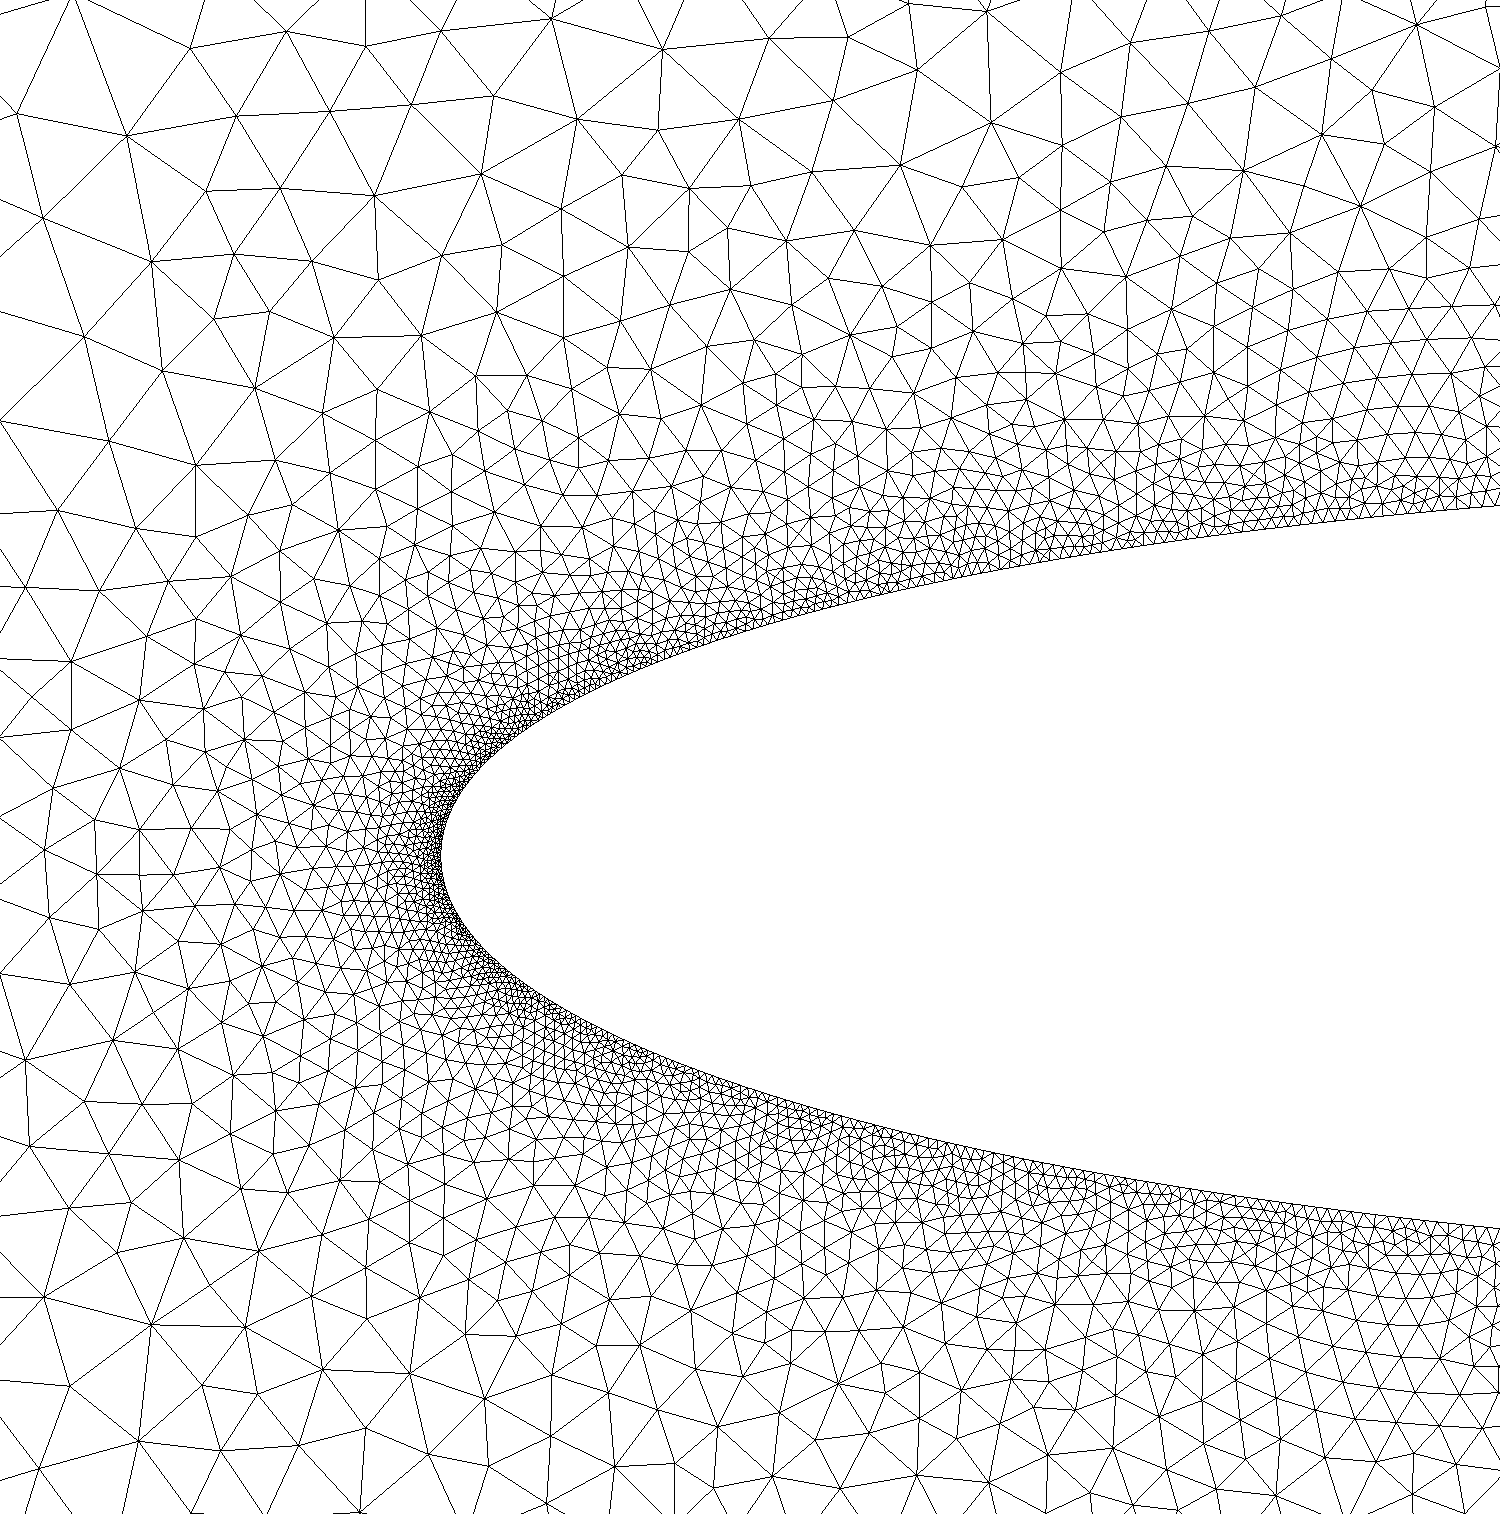
\includegraphics[width=\linewidth]{\mainpath/fig/geo/bodyfitted.png}
			        \caption{classical wall boundary}
			    \end{subfigure}~
			    	\begin{subfigure}[t]{0.4\textwidth}
			        \centering
			        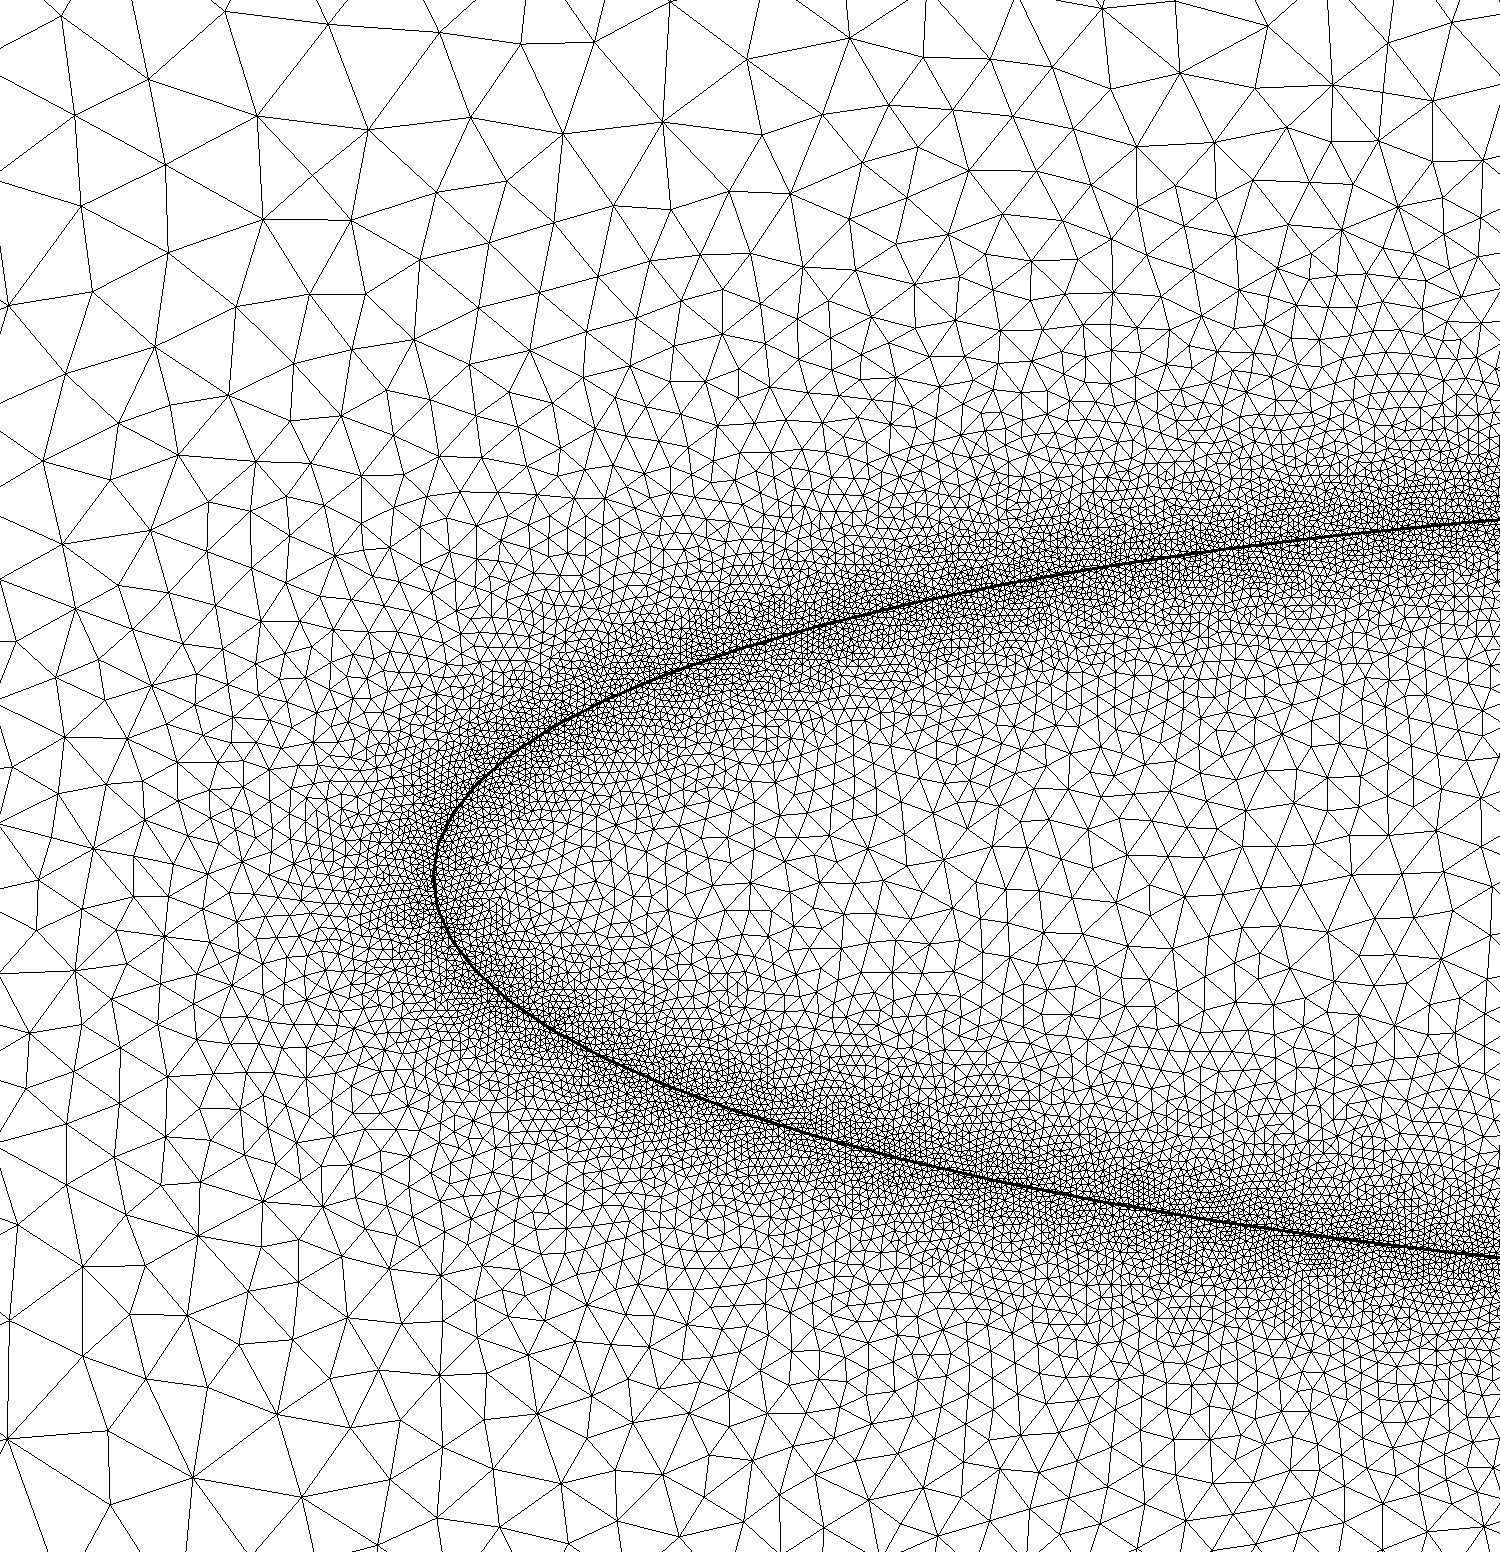
\includegraphics[width=\linewidth]{\mainpath/fig/geo/embedded.png}
			        \caption{immersed wall boundary}
			    \end{subfigure}%
\caption[Visualization of immersed boundary method versus embedded boundary method]{NACA 0012 profile meshed with a classical wall boundary on the left versus an immersed boundary on the right. This geometry is relatively simple, for more complex examples, however, not requiring a conforming fluid grid on the interface can be a huge advantage.}
\label{fig:ale_vs_embedded}
\end{figure}




\end{document}
